% This must be in the first 5 lines to tell arXiv to use pdfLaTeX, which is strongly recommended.
\pdfoutput=1
% In particular, the hyperref package requires pdfLaTeX in order to break URLs across lines.

\documentclass[11pt]{article}

% Remove the "review" option to generate the final version.
\usepackage[final]{ACL2023}

% Standard package includes
\usepackage{times}
\usepackage{latexsym}

% For proper rendering and hyphenation of words containing Latin characters (including in bib files)
\usepackage[T1]{fontenc}
% For Vietnamese characters
% \usepackage[T5]{fontenc}
% See https://www.latex-project.org/help/documentation/encguide.pdf for other character sets

% This assumes your files are encoded as UTF8
\usepackage[utf8]{inputenc}

\usepackage{graphicx}

% This is not strictly necessary, and may be commented out.
% However, it will improve the layout of the manuscript,
% and will typically save some space.
\usepackage{microtype}

% This is also not strictly necessary, and may be commented out.
% However, it will improve the aesthetics of text in
% the typewriter font.
\usepackage{inconsolata}


% If the title and author information does not fit in the area allocated, uncomment the following
%
%\setlength\titlebox{<dim>}
%
% and set <dim> to something 5cm or larger.

\title{Social Media Monitoring}

\author{Aysenur Kocak \\
  Technical University \\ of Munich \\
  \texttt{aysenur.kocak@tum.de} \\\And
  Youssef Lotfy \\
  Technical University \\ of Munich \\
  \texttt{ge92zaq@mytum.de} \\\And
  Leonhard Stengel \\
  Technical University \\ of Munich \\
  \texttt{leonhard.stengel@tum.de} \\}

\begin{document}
\maketitle
\begin{abstract}
Event detection on social media platforms, particularly Twitter (now known as X), is critical for fields like journalism, public safety, and crisis management. This project implements a social media monitoring module within the Automated Journalist App to automatically detect and cluster relevant events with minimal human intervention. Leveraging key components of the EDT\textsubscript{BERT} model by \citet{edtbert}, we represent tweets as nodes in a graph, using structural and contextual similarities to identify clusters with the Markov Clustering (MCL) method. We then summarize these clusters using Google's FLAN-T5 model, producing concise summaries for seamless news integration. Our system achieves a precision of 85\%, a recall of 70\%, and an F1-score of 77\% on the Event2012 dataset, highlighting its effectiveness in real-time social media monitoring and its contribution to automated journalism.
\end{abstract}

% INTRODUCTION
\section{Introduction}
The rapid proliferation of social media platforms, particularly Twitter (now known as X), has revolutionized the way information is disseminated and consumed globally. Social media serves as a real-time pulse of public opinion, breaking news, and emerging trends, making it a vital source of information for various fields, including journalism, public safety, crisis management, and disaster response. The vast and dynamic nature of social media content, however, presents significant challenges in identifying and summarizing relevant events effectively.

Automated journalism, which aims to generate news content from structured data with minimal human interference, has emerged as a promising solution to these challenges. Central to this concept is the ability to monitor social media, detect relevant events in real-time, and generate accurate, concise summaries that can be used directly in news reporting. This paper presents our work on developing the Social Media Monitoring module that integrates with the Automated Journalist App, designed to automatically detect and cluster events from social media data.

Our work builds on the EDT\textsubscript{BERT} framework by \citet{edtbert}, incorporating both structural and contextual embeddings to preprocess tweets and represent them as nodes in a graph, with edges denoting similarities. By applying the Markov Clustering (MCL) algorithm \cite{mcl}, we identify clusters of related tweets, which represent potential events. To further enhance the system's utility, we use a large language model (LLM) to generate summaries of these clusters, making the detected events more accessible and actionable for automated news generation.

Our approach is evaluated using the Event2012 dataset, where it achieves a precision of 85\%, a recall of 70\%, and an F1-score of 77\%, demonstrating the system's robustness and effectiveness in real-time event detection. This work significantly contributes to the field of automated journalism by providing a reliable method for real-time social media monitoring and event summarization.

The Social Media Monitoring project was a collaborative effort by the authors of this paper. Aysenur Kocak was responsible for implementing Contextual Embeddings (Section \ref{sec:contextualembeddings}), Graph Clustering (Section \ref{sec:graphclustering}), and Event Summarization (Section \ref{sec:eventsummarization}). She also conducted research on BERT-Based Event Detection (Section \ref{sec:bertbased}) and led the compilation of the poster and the report. Youssef Lotfy was responsible for implementing Structural Embeddings (Section \ref{sec:structuralembeddings}), Dashboard (Section \ref{sec:dashboard}) and code documentation. He also conducted research on Graph-Based Event Detection (Section \ref{sec:graphbased}). Leonhard Stengel ensured code quality and was responsible for the implementations of Preprocessing (Section \ref{sec:preprocessing}), Graph Construction (Section \ref{sec:graphconstruction}), and Integration to the Automated Journalist App (Section \ref{sec:integration}). He also conducted research on Clustering-Based Event Detection methods (Section \ref{sec:clusteringbased}).

% RELATED WORK
\section{Related Work}
Event detection on social media platforms, particularly Twitter, has been extensively studied using various approaches, including clustering-based, BERT-based, and graph-based methods. Each of these methodologies offers unique strengths in addressing the challenges of real-time event detection from noisy and unstructured social media data.

\subsection{Clustering-Based Event Detection}
\label{sec:clusteringbased}
Clustering methods have been widely used for real-time event detection, where tweets are grouped based on their similarities. \citet{becker2011beyond} proposed a model that represents each post as a tf-idf weight vector and applies an incremental clustering algorithm to identify event-related clusters, achieving an F1-score of 0.837 on their dataset. \citet{li2017real} introduced a method that clusters tweets first by retweets and links, then by embeddings on semantic classes, using cosine similarity and tf-idf as similarity measures. \citet{kolajo2022real} developed the Social Media Analysis Framework for Event Detection (SMAFED), which employed histogram-based incremental clustering (SHC) on the Event2012 Twitter dataset. 

\subsection{Graph-Based Event Detection}
\label{sec:graphbased}
Graph-based methods are another prominent approach, where tweets are represented as nodes in a graph, and edges indicate relationships or similarities, such as shared hashtags or keywords. The graph is then clustered using clustering algorithms such as the Louvain method or spectral clustering to identify event-related clusters. \citet{graphclus} proposed a graph-based method for real-time event detection from Twitter. In their method, tweets are vectorized using tf-idf formula. A tweet graph is constructed, where nodes represent tweet vectors and edges between nodes represent the cosine similarity between two tweet vectors. Then, the well-known MCL algorithm is applied to identify events. \citet{singh2024event} utilized the Louvain community detection algorithm on a graph representation of keywords extracted from tweets, achieving an F1-score of 0.84.

\subsection{BERT-Based Event Detection}
\label{sec:bertbased}
The application of BERT (Bidirectional Encoder Representations from Transformers) \cite{bert} in event detection has gained traction due to its ability to capture deep contextual information from text. \citet{bertweet} developed BERTweet, a pre-trained language model specifically designed for English tweets, which significantly improved performance on various tweet-based NLP tasks.  \citet{edtbert} proposed EDT\textsubscript{BERT}, a model that combines structural and contextual information to represent tweets as nodes in a graph, employing the Markov Clustering Algorithm (MCL) \cite{mcl} to identify event clusters. \citet{eventbert} introduced EventBert, a pre-trained model designed for event correlation reasoning, further enhancing the understanding of event sequences in natural language texts.


These approaches highlight the diversity of techniques employed in event detection from social media, each contributing valuable insights and methodologies to the field. Our work builds on these foundations, integrating elements from BERT-based and graph-based methods to develop a robust system for real-time event detection and summarization.

% METHODOLOGY

\section{Methodology}

In this study, word affinity has been determined by examining temporal correlation, structural characteristics, and semantic similarity. To establish temporal coherence, the received tweets are divided into several time intervals according
to their chronological order. Tweets within a specified time window are analyzed in order to detect events. The Event Detection Task starts with constructing a graph of tweets to model the structural and contextual relationships
among tweets. Specifically, the BERT sentence encoder is utilized to find tweet embeddings and overlapping named entities, and hashtags are used to find structural associations among tweets. Then, the MCL graph clustering algorithm is employed to find semantically similar tweet clusters related to an event. In this study, a threshold of 0.29 is used to control the granularity of the clustering process within the MCL algorithm. These clusters are then summarized by extracting key terms and generating concise summaries using Google’s FLAN-T5 model. Additionally, clusters are classified into topics using a pre-trained model, with results visualized through a pie chart. The final output includes cluster summaries, keywords, topics, and cluster sizes, contributing to the automated detection and reporting of events. The process is integrated with a dashboard and the Automated Journalist App, enabling efficient end-to-end event monitoring and reporting.

\begin{figure}[htbp]
    \centering
    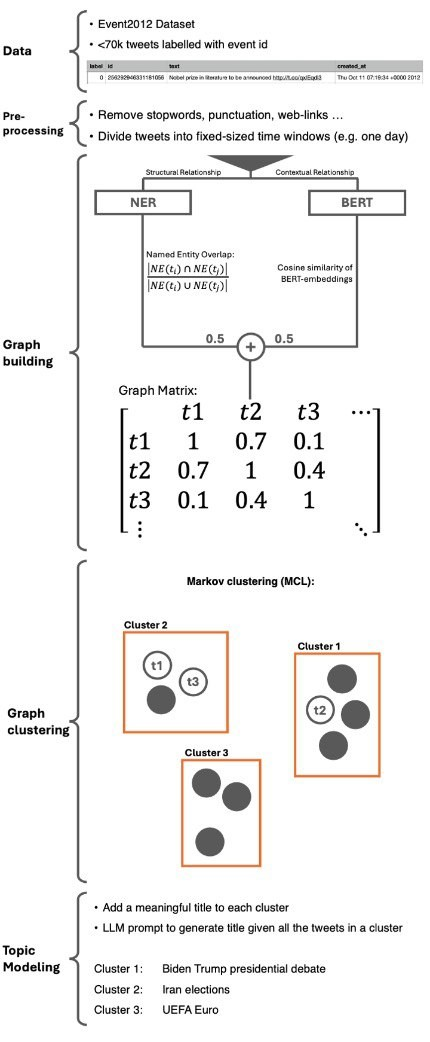
\includegraphics[width=0.95\linewidth]{Images/model.jpeg}
    \caption{Overview of the Social Media Monitoring Pipeline}
    \label{fig:model}
\end{figure}

As shown in Figure \ref{fig:model}, the process involves multiple stages including data preprocessing, graph building, and topic modeling.

\subsection{Preprocessing}
\label{sec:preprocessing}
The preprocessing stage is essential for cleaning and preparing tweets before further analysis. The process involves the following steps:
\begin{itemize}
\item Lowercasing: All tweets are converted to lowercase to ensure uniformity in text analysis.

\item Tokenization: Tweets are tokenized using the TweetTokenizer from the NLTK library\footnote{\url{https://www.nltk.org/}}, which is specifically designed to handle social media text.

\item Removing Short Tweets: Tweets with fewer than three words are discarded, as they are unlikely to provide meaningful information.

\item Stopword Removal: Common stopwords are removed from the tweets to focus on more informative words.

\item Web Links Removal: Web links starting with "http" or "www" are removed from the tweets, as they often add noise to the data.

\item Punctuation Removal: Punctuation marks are removed from tokens, except for hashtags, which are retained for their relevance in social media contexts.

\item Non-ASCII Characters Removal: Non-ASCII characters are removed to avoid encoding issues during further processing.

\item Retweet Removal: Retweets can be filtered out as needed, although this step is currently optional in the implementation.

\item Cleaning Empty Tokens: Any remaining empty tokens are removed to ensure clean data.
\end{itemize}
After normalization, only tweets that have been successfully processed and contain meaningful content are retained for further analysis. This preprocessing ensures that the data used in the subsequent stages is clean, consistent, and relevant for event detection.

\subsection{Graph Construction}
\label{sec:graphconstruction}
In the graph construction module, tweets are processed and modeled as a graph, where nodes represent tweets and edges represent the similarities between tweets. This similarity computation is crucial for clustering tweets related to specific events. In this study, we use the similarity metric proposed by \citet{edtbert} in the EDT\textsubscript{BERT} model, that is designed to capture both the structural associations and contextual relationships between tweets.

\subsubsection{Contextual Embeddings}
\label{sec:contextualembeddings}
In order to capture contextual knowledge, it is essential to convert textual input into vector representations, which can then be used to calculate the similarity between tweets. Various embedding techniques, such as One-Hot Encoding and Term Frequency Inverse Document Frequency (TFIDF), can be employed for this purpose. However, not all techniques are capable of adequately capturing the contextual nuances present in tweets. To address this, a pre-trained BERT sentence transformer \citep{sentence-bert} was utilized, specifically the all-mpnet-base-v2\footnote{\url{https://huggingface.co/sentence-transformers/all-mpnet-base-v2}} model, to encode the preprocessed tweets. Each tweet is passed through the BERT embedding module, resulting in a dense 768-dimensional vector. The contextual similarity between tweet vectors is then calculated using the cosine similarity measure. In the graph of tweets, each node represents a tweet as a 768-dimensional BERT embedding vector, and edges connect tweets if their semantic similarity exceeds a predefined threshold (in the experiment, the threshold is set to 0.29). The Structural Relation (SR) and Contextual Similarity (CS) are given equal weight in our approach, as done in the EDT\textsubscript{BERT} model.


\subsubsection{Structural Embeddings}
\label{sec:structuralembeddings}
To establish structural relationships, the graph construction also considers the overlap of hashtags and named entities (NEs) between tweets. These overlaps indicate the formation of cliques, where tweets are interconnected due to their association with common events. The degree of overlap in hashtags and named entities between two tweets is calculated using the Jaccard Similarity measure. This measure is used to quantify the structural similarity between tweets, with the structural relationship between two tweets being a combination of their hashtag overlap and named entity overlap.

\subsection{Graph Clustering}
\label{sec:graphclustering}
Using the structural relationship and contextual knowledge, a tweet graph is generated from preprocessed tweets. And the tweet graph is passed to the next module for the event detection task. In this study, the Markov clustering (MCL) method \cite{mcl} is used to analyze the graph representation of tweets, aiming to detect clusters of related tweets. The MCL algorithm has the capability to split the graph into clusters without requiring the number of clusters to be specified as an input parameter. The methodology employed in this technique is based on the idea that clusters are present inside a given graph. It utilizes a random walk approach to aid the process of clustering.



\subsection{Event Summarization}
\label{sec:eventsummarization}
The event summarization component of the Social Media Monitoring system is designed to generate concise and informative descriptions of detected event clusters on social media. This component combines traditional natural language processing (NLP) techniques with state-of-the-art large language models (LLMs) to produce meaningful summaries of event-related tweet clusters.

\subsubsection{Top Words Extraction} For each detected cluster, the most salient keywords that characterize the cluster are extracted. Tweets within each cluster are preprocessed and represented in a term-document matrix, allowing the identification of the most frequently occurring unigrams, bigrams, and trigrams. This process is facilitated using the CountVectorizer from the scikit-learn\footnote{\url{https://scikit-learn.org/stable/}} library. The extracted top words provide a preliminary summary of the cluster's content, highlighting the core topics being discussed.

\subsubsection{Cluster Summarization} To generate more comprehensive summaries, Google's FLAN-T5 \cite{google-flan-t5}, a transformer-based sequence-to-sequence model, is employed. The top words from each cluster serve as prompts for the model, which then generates a concise textual summary that encapsulates the primary themes of the cluster. This method ensures that the generated summaries are both coherent and contextually relevant, making them suitable for integration into automated news content generation. In this study, google/flan-t5-base\footnote{\url{https://huggingface.co/google/flan-t5-base}} model is used.

\subsubsection{Topic Detection} In addition to summarization, the overarching topic of each cluster is classified using a pre-trained topic classification model tailored for Twitter content. This model assigns clusters to predefined categories such as "arts \& culture," "business \& entrepreneurs," "pop culture," "daily life," "sports \& gaming" and "science \& technology." The classification is performed using a transformer-based model cardiffnlp/tweet-topic-latest-single\footnote{\url{https://huggingface.co/cardiffnlp/tweet-topic-latest-single}} developed by \citet{twitter-topic-classification}, which outputs the most likely topic based on the content of the tweets in each cluster. The distribution of topics across clusters is visualized using a pie chart, providing insights into the dominant themes in the detected events, as shown in the Figure \ref{fig:pie_chart}.

\begin{figure}[htbp]
    \centering
    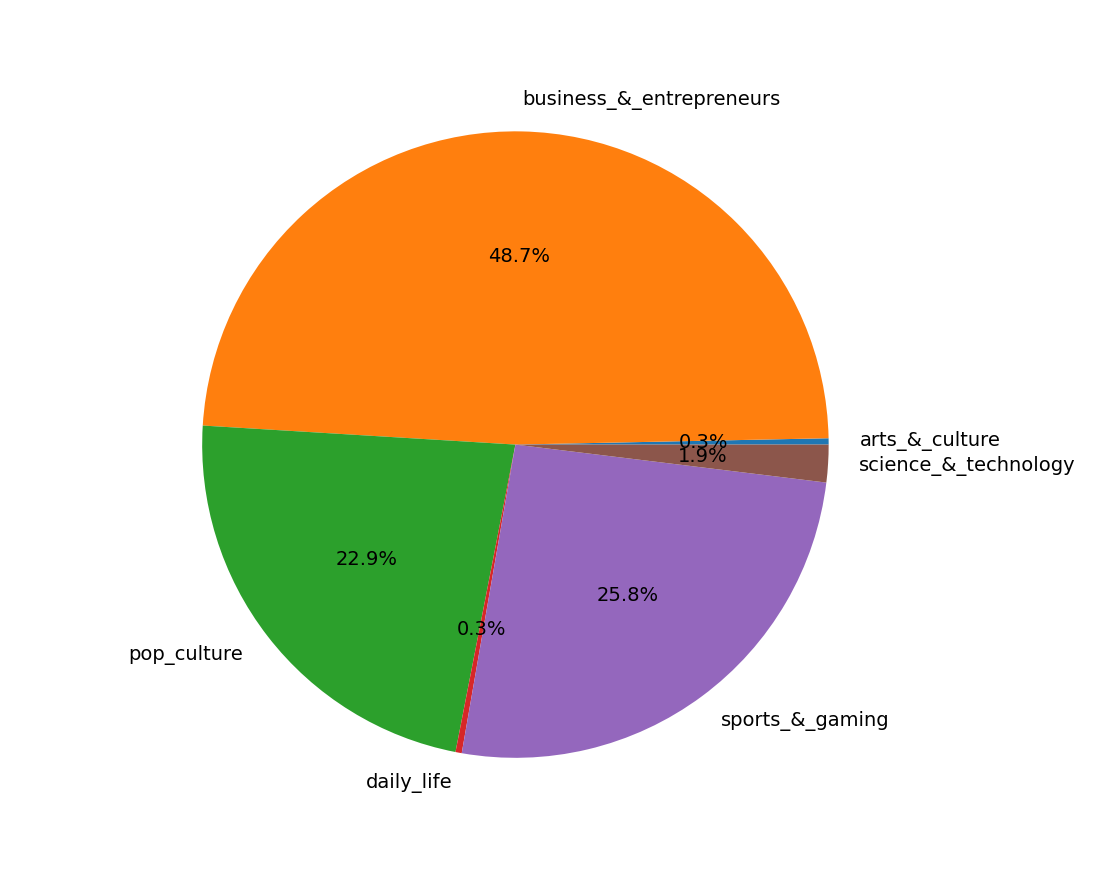
\includegraphics[width=1\linewidth]{Images/pie_chart.png}
    \caption{Distribution of Tweet Topics}
    \label{fig:pie_chart}
\end{figure}

\subsubsection{Output} The final output of the event summarization module includes a detailed summary for each cluster, a list of the most relevant keywords, the identified topic, and the size of the cluster. This output is crucial for understanding the context and significance of the detected events. 

By integrating advanced NLP techniques with LLMs, the event summarization component enhances the automated detection and reporting of social media events, contributing to the overall goal of producing high-quality, automated news content.

\subsection{Dashboard Implementation} 
\label{sec:dashboard}
The Event Monitoring Dashboard provides a visual interface for users to explore detected events and their relevance. Implemented using Streamlit\footnote{\url{https://streamlit.io/}}, the dashboard enables users to visualize the clustering results, facilitating a better understanding of how events are grouped based on structural and contextual similarities, as shown in the Figure \ref{fig:dashboard}.

\begin{figure}[htbp]
    \centering
    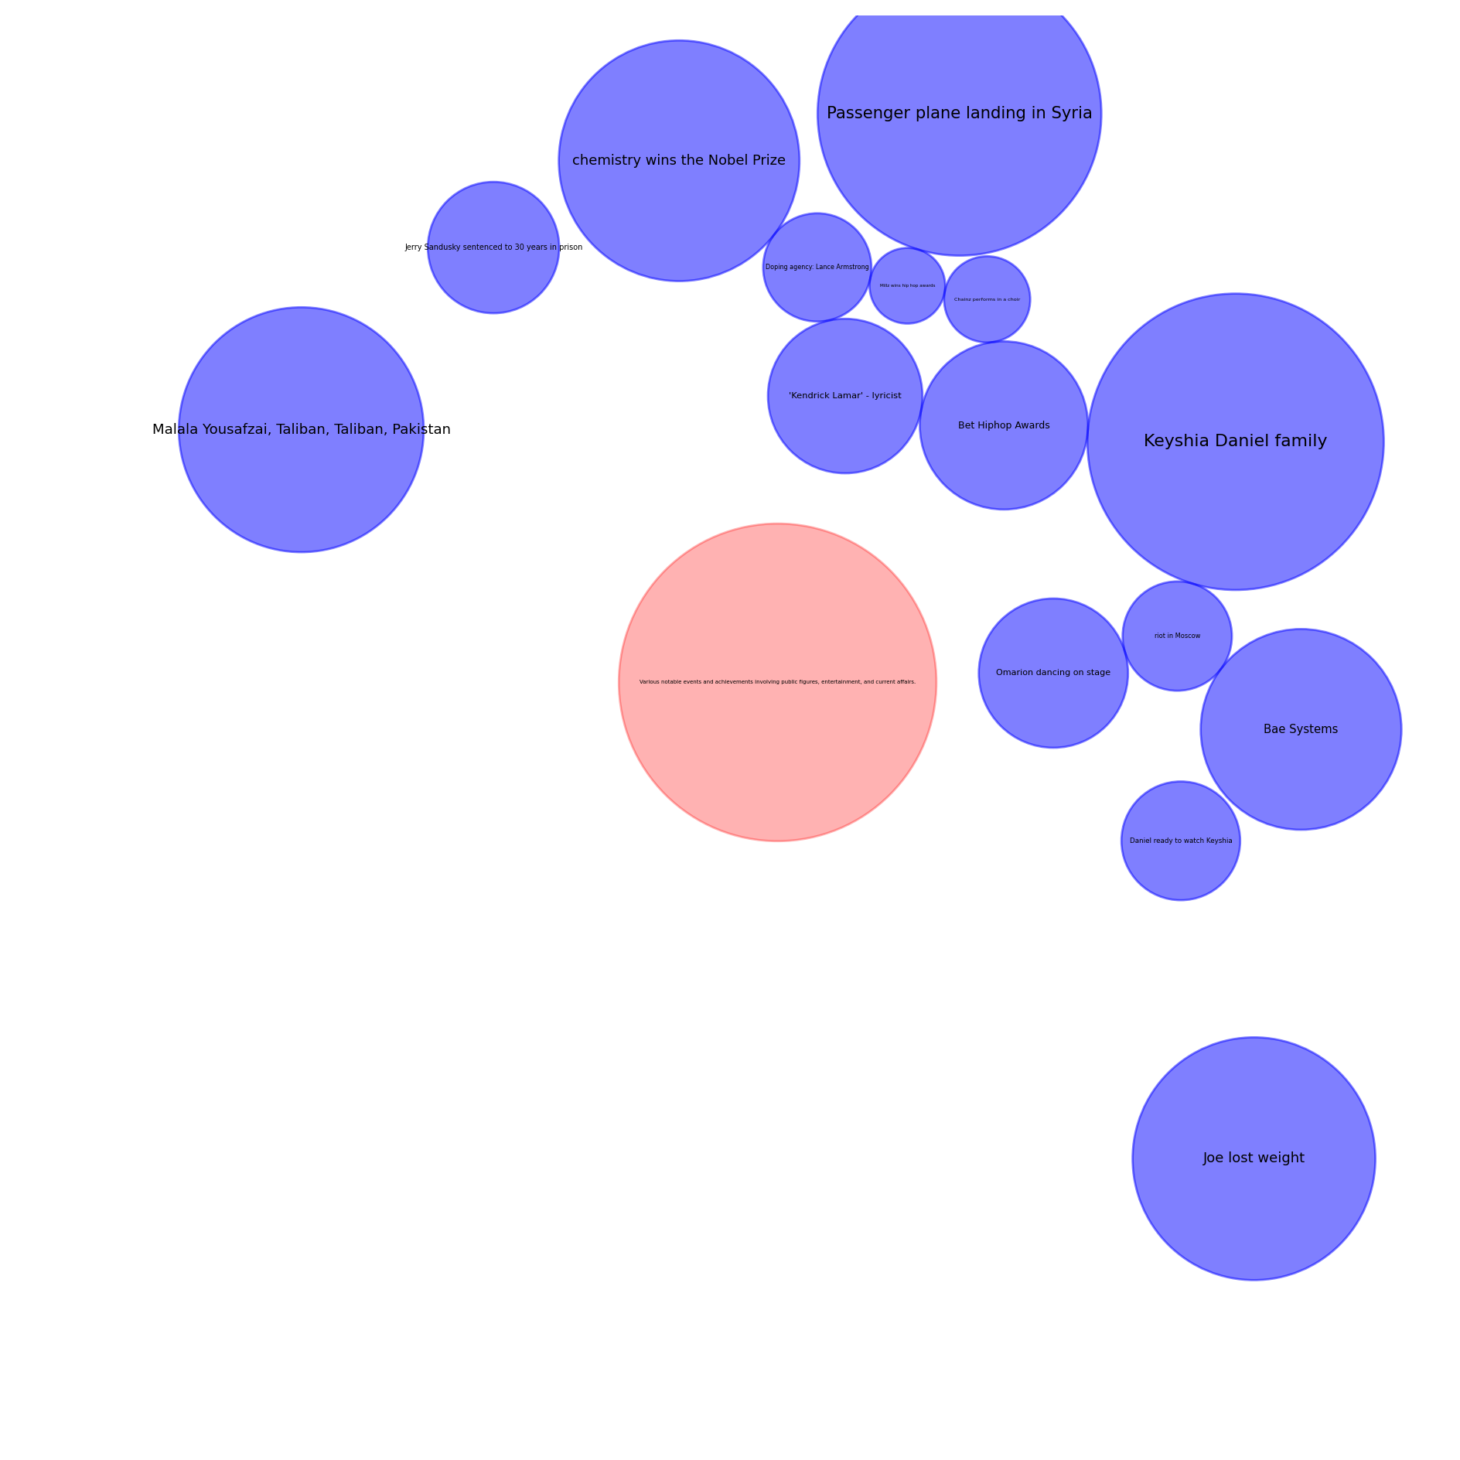
\includegraphics[width=1\linewidth]{Images/dashboard.png}
    \caption{Visualization of the Clusters}
    \label{fig:dashboard}
\end{figure}
\subsubsection{Data Preparation} 
The dashboard begins by setting up the page layout to be wide, ensuring that the visualization can utilize the full screen space available. The key input to this dashboard is a preprocessed dataset containing tweet summaries, which is loaded from a JSON file. This dataset is converted into a pandas DataFrame for ease of manipulation and display.

\subsubsection{Event Representation and Similarity Calculation}  

To identify the relevance of events, the dashboard employs vectorization techniques. Using the Sent2Vec\footnote{\url{https://pypi.org/project/sent2vec/}} vectorizer, each tweet summary, along with a predefined query, is converted into vector embeddings. These vectors are used to compute the cosine similarity between the query and each tweet summary, allowing us to measure how closely each summary aligns with the topic of interest.

\subsubsection{Visualization: Mapping Similarity to a 2D Plane}   

The dashboard visualizes the similarity between events by mapping these values onto a 2D plane. This is achieved by normalizing the similarity scores and then using trigonometric functions (cosine and sine) to generate coordinates for each event. The resulting 2D coordinates are scaled to fit within a defined range, ensuring that all events are visually distinguishable.

\subsubsection {Radius Calculation and Overlap Resolution}

Each event is represented as a circle, with the radius corresponding to the size of the event cluster. Larger clusters are depicted with larger circles, signifying their importance. To avoid overlapping circles, an iterative algorithm is implemented to adjust the positions of circles that overlap, ensuring a clear and uncluttered visualization.

\subsubsection {Plotting and Display}

The dashboard then draws these circles on a matplotlib plot, annotating each with the event summary. A central circle represents the query topic, serving as a reference point for the related events. The plot is carefully configured to maintain aspect ratio and avoid distortion, and the axes are turned off to emphasize the event clusters visually.


\subsection{Integration to the Automated Journalist App}
\label{sec:integration}
The integration of the event detection functionality into the existing Automated Journalist App aims to enhance its capabilities by identifying significant events from social media posts retrieved by a user query. The primary objective is to detect these events and visualize them using the developed dashboard. For this purpose, an Event Detection Module has been constructed, consisting of a Flask\footnote{\url{https://flask.palletsprojects.com/en/3.0.x/}} Backend and a Streamlit Frontend. Both must be run in parallel with the Automated Journalist App. The Flask Backend offers two API endpoints: "update-events", which receives social media posts from the automated journalist app to execute the event detection process, and "/events", which returns the list of current events detected. The Streamlit Frontend proactively requests the current events from the "/events" endpoint every five seconds to ensure that the dashboard remains up-to-date with the latest information. To facilitate this integration seamlessly, a "Detect Events" button has been added to the feed of the Automated Journalist App. When clicked, the button sends the current feed to the event detection backend, triggering the event detection process, and subsequently, the Streamlit Frontend presents the updated dashboard to the user, showcasing the detected events in real-time. A screenshot from the Automated Journalist App is shown in the Figure \ref{fig:integration}.

\begin{figure}[htbp]
    \centering
    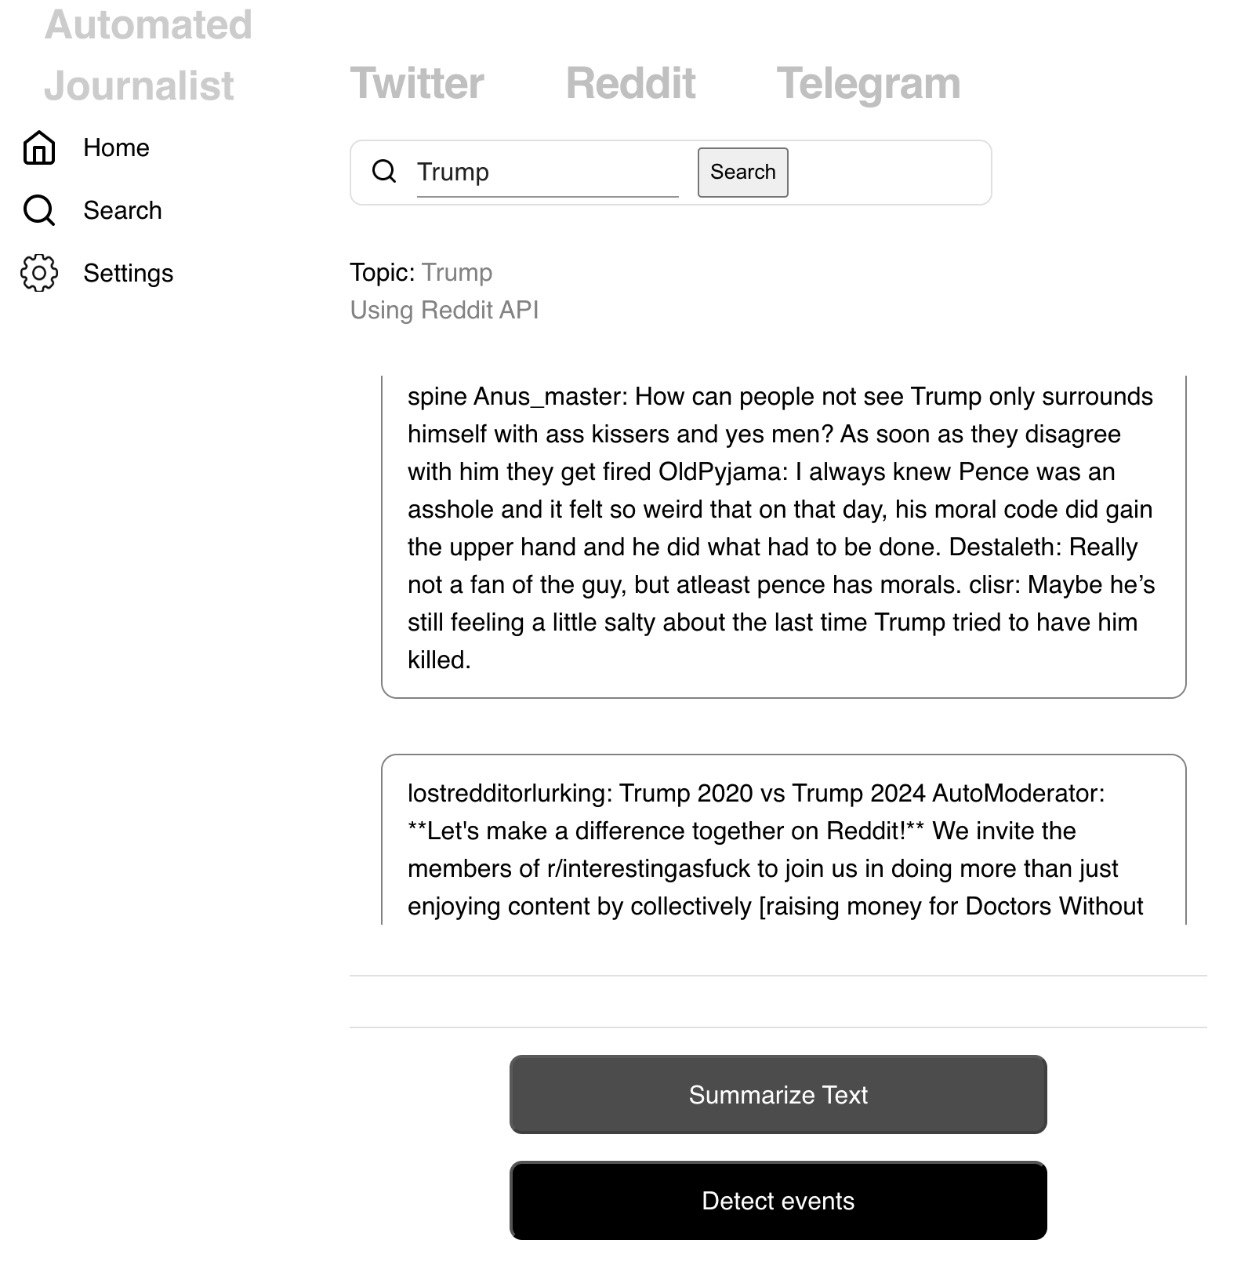
\includegraphics[width=0.95\linewidth]{Images/integration.jpeg}
    \caption{Social Media Monitoring module integrated into the Automated Journalist App}
    \label{fig:integration}
\end{figure}

% EXPERIMENTS
\section{Experiments}
Most event detection solutions have historically been developed and tested using Twitter data due to its real-time nature and extensive user base. Following this, we also evaluated our approach using tweets. However, there was a significant problem: Twitter’s policies do not allow sharing of tweet datasets with the tweet texts, only tweet IDs. Furthermore, accessing tweets through the Twitter API proved financially unfeasible. Fortunately, we discovered an unofficial dataset containing over 70,000 tweets, each labeled with the creation date, time, and a event the tweet is about. Before evaluation, we preprocessed the data by removing duplicates and converting the dataset into a CSV format. This enabled us to carry out an evaluation of the EDT\textsubscript{BERT} implementation on this dataset. To evaluate the clustering results, we used precision, recall, and F1 scores, which are essential metrics for determining the accuracy of classification systems. For each pair of tweets, clustering results were compared: if both tweets were in the same cluster and matched the ground truth, they were counted as True Positive; if in different clusters and correctly so in the ground truth, as True Negative. Conversely, mismatches were counted as False Positives or Negatives. Using these criteria, we calculated the precision, recall, and F1 score, providing a assessment of our model’s performance.

% RESULTS & DISCUSSIONS
\section{Results \& Discussion}
The results of our study demonstrate the effectiveness of our Social Media Monitoring module, particularly in detecting and clustering relevant events from Twitter data in real-time. We evaluated our system on the Event2012 dataset. The system achieved a precision of 85\%, a recall of 70\%, and an F1-score of 77\%, which are comparable to or exceed the performance of previous state-of-the-art methods.
\subsection{Precision, Recall, and F1-Score}
The high precision (85\%) indicates that the system is highly accurate in identifying true events from the tweet clusters, with minimal false positives. This precision is crucial in applications like automated journalism, where the accuracy of detected events directly impacts the quality of the generated news content. The recall of 70\%, while slightly lower, suggests that the system is reasonably effective at capturing a wide range of events, though some relevant events might be missed, which is an area for potential improvement. The F1-score of 77\% reflects a balanced performance, combining both precision and recall into a single metric that underscores the robustness of our approach.
\subsection{Event Summarization and Utility}
The event summarization module, powered by Google’s FLAN-T5 model, effectively condensed the tweet clusters into concise and informative summaries. This is particularly valuable for automated journalism, where the speed and clarity of reporting are paramount. The summaries generated were coherent and contextually relevant, often capturing the essence of the events with minimal extraneous information. This level of summarization ensures that the outputs are not only accurate but also actionable, providing journalists and end-users with clear insights into emerging trends and breaking news.

\subsection{Dashboard and User Interaction}
The integration of the Event Detection Module with the Automated Journalist App, along with the implementation of a user-friendly dashboard, significantly enhances the utility of the system. The dashboard's ability to visualize events and their relevance in real-time offers users an intuitive way to monitor and assess the significance of detected events. The iterative algorithm for overlap resolution in visualization ensures that users can easily distinguish between different event clusters, improving the overall user experience.

\subsection{Challenges and Limitations}
Despite the system’s strengths, there are several challenges and limitations that warrant discussion. One of the main limitations is the reliance on a fixed threshold for similarity measures, which may not be universally optimal across different types of events or datasets. Future work could explore adaptive thresholding mechanisms to enhance flexibility and accuracy. Additionally, the recall rate suggests that some relevant events may be overlooked, possibly due to the granularity of clustering or the inherent noise in social media data. Addressing these issues may involve refining the preprocessing steps or exploring alternative clustering algorithms.

Another challenge was the dependency on tweet data for evaluation, as Twitter’s policy restrictions posed limitations on accessing and sharing comprehensive datasets. This constraint necessitated the use of unofficial datasets, which, while effective, may not fully capture the diversity and dynamics of real-world social media environments.



% CONCLUSION
\section{Conclusion}

In conclusion, the Social Media Monitoring module developed for the Automated Journalist App represents an exploration of methodologies in automated event detection and summarization. While it leverages established techniques like graph-based clustering and large language models, the project serves primarily as a practical investigation into how these methods can be applied to real-time social media data. The module achieved respectable results in terms of precision, recall, and F1-score on the Event2012 dataset, demonstrating its potential utility. However, there remains significant room for improvement, particularly in handling the complexities and noise inherent in social media data. This work lays a foundation for further refinement and testing, with the aim of developing more robust and reliable tools for automated journalism in the future.

% REFERENCES
\bibliography{bibliography}
\bibliographystyle{acl_natbib}

% APPENDIX (OPTINAL)

\end{document}
